\documentclass{cheatsheet}
\usepackage{bm}
\usepackage{textcomp, mathcomp}
\usepackage{empheq}
\usepackage{pbox}
\usepackage{booktabs}

\doctitle{Physik Zusammenfassung}
\author{Noa Sendlhofer \& Christian Leser \\ nsendlhofer \& cleser \\ \vspace*{-0.2em}}

\begin{document}
\section{1. Elektrizitätslehre}
    \subsection*{1.1 Definition Strom}

\begin{itemize}
    \item Ladungen mit gleichem Vorzeichen stossen sich ab.
    \item zwei unendlich lange parallele Drähte im Abstand 1 m voneinander, die von einem Strom von 1 A gleichsinnig durchflossen werden, ziehen sich mit einer Kraft von $2 \cdot 10^{-7} N$ pro Meter Leiterlänge an.
    \item Elementarladung: $e = 1.602 \cdot 10^{-19}$
\end{itemize}


Stromstärke: \mathbox{I = \frac{dQ}{dt}}
Ladung: \mathbox{Q = \int\limits_{\Delta t} I dt}
Widerstand: \mathbox{R = \frac{U}{I}, I \sim U}

\begin{tabular}{c c}
    Ohmsche Leiter & nicht-ohmsche Leiter \\
    $I = \frac{U}{R}$ & $R_{\text{diff}} = \frac{dU}{dI}$\\
    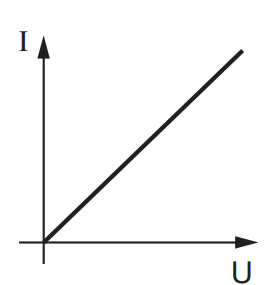
\includegraphics[width = 30mm]{src/images/plot_ohmscher_leiter.png} & 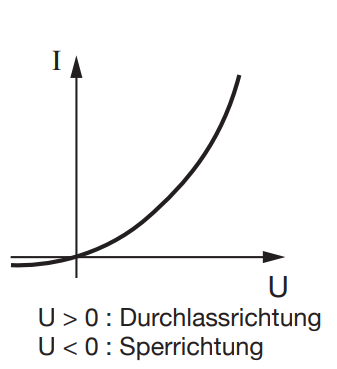
\includegraphics[width = 30mm]{src/images/plot_nicht-ohmscher_leiter.png}
\end{tabular}


    \subsection*{1.2 Klassifizierung ohmscher Leiter}
nach Grösse:
\mathbox{R = \rho \frac{l}{A}}, l Leiterlänge, A Leiterquerschnitt, $\rho$ spezifischer Widerstand
Spezifische Leitfähigkeit: $ K = \frac{1}{\rho}$\\
nach Temperatur:
\mathbox{\rho(T)}
    \subsection*{1.3 Kirchhoffsche Regeln}
    \subsubsection*{Knotenregel}
    \mathbox{\sum\limits_k I_k = 0}

    \subsubsection*{Maschenregel}
    \mathbox{\sum\limits_i U_i = \sum\limits_k I_k R_k}

    \subsubsection*{Serieschaltung}
    \[
        U_0 = I \cdot R_{tot} = I \cdot \left(\sum\limits_i R_i\right) \Rightarrow \boxed{R_{tot} = \sum\limits_i R_i}
    \]

    \subsubsection*{Parallelschaltung}
    \[
        I_{tot} = \frac{U}{R_{tot}} = \sum\limits_i \frac{U}{R_i} \Rightarrow \boxed{\frac{1}{R_{tot}} = \sum\limits_i \frac{1}{R_i}}
    \]

\section{2. Elektrisches Feld}
    \subsection{2.1 Feldlinien}
    Elektrisches Feld immer tangential an Feldlinie
    \begin{tabular}{c c c}
        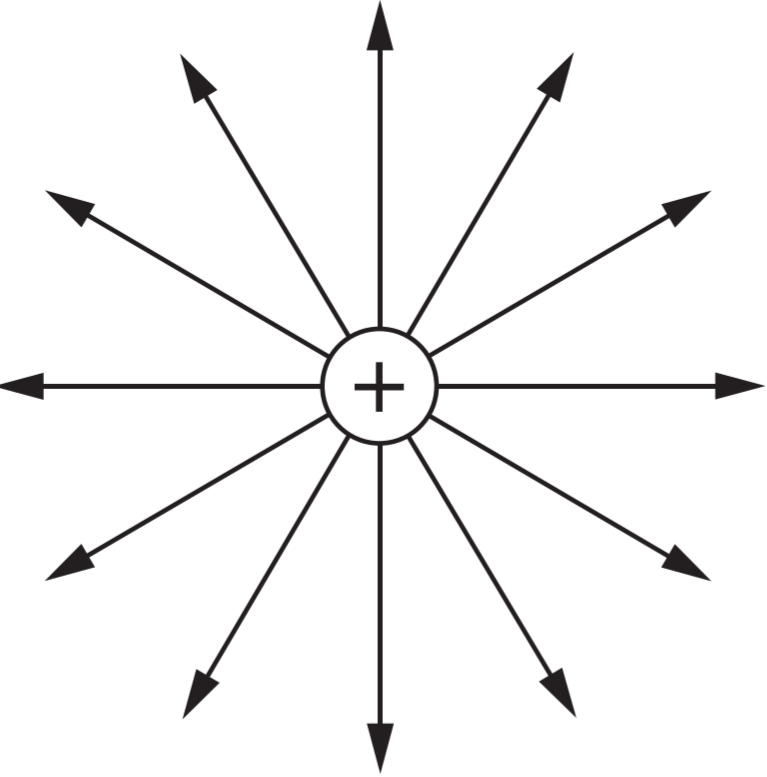
\includegraphics[height = 20mm]{src/images/punktladung.png} & 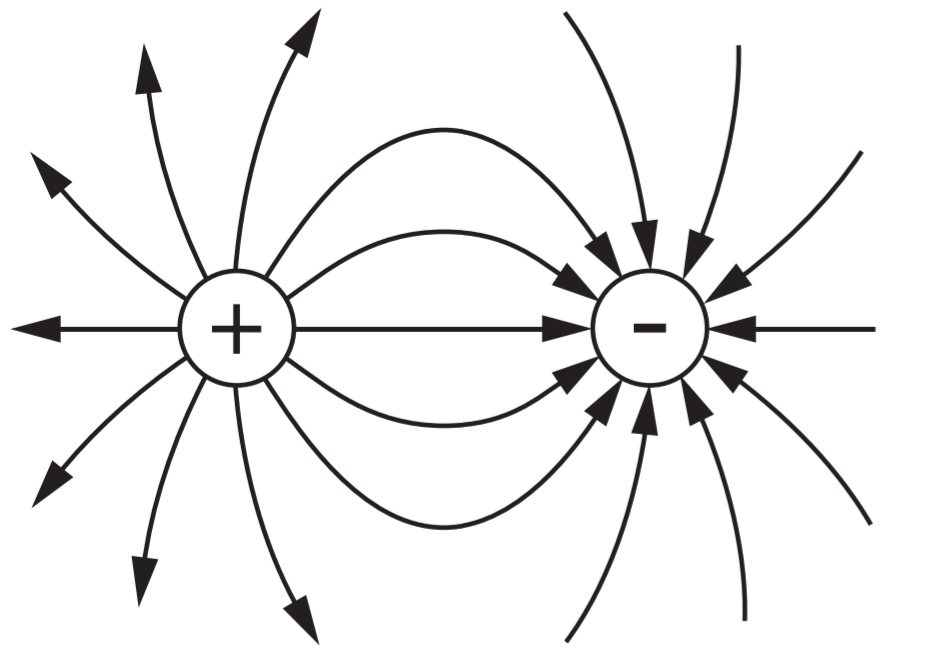
\includegraphics[height = 20mm]{src/images/zwei_punktladung.png} & 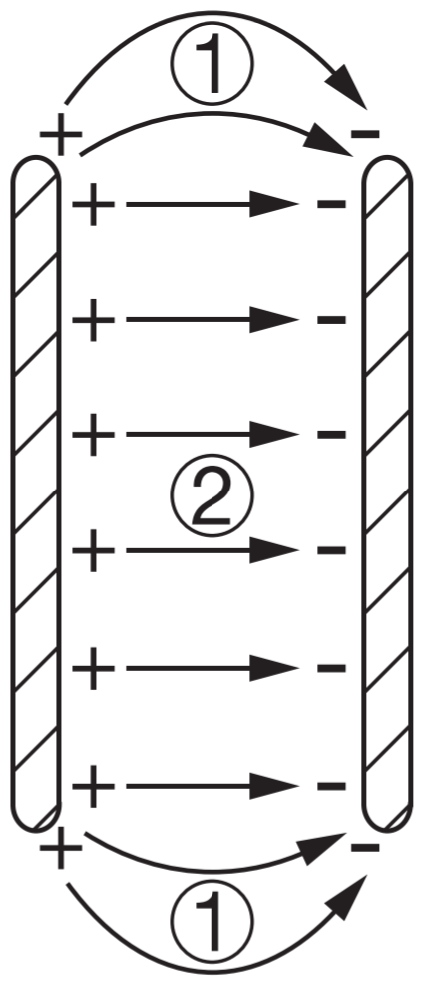
\includegraphics[height = 30mm]{src/images/kondensator.png}
    \end{tabular}

    \subsubsection*{Elektrische Feldstärke}
        \mathbox{\overrightarrow{E} = \frac{U}{l} \overrightarrow{e}} mit e Einheitsvektor in Richtung der Feldlinien

    \subsubsection*{Verschiebungsdichte bzw. Flussdichte}
        Dichte der Ladung:
        \mathbox{\overrightarrow{D} = \frac{Q}{A} \overrightarrow{e}}
        Im Vakuum: $\overrightarrow{D} = \varepsilon_0 \cdot \overrightarrow{E}$\\

\section{3. Magnetisches Feld}

\section{4. Elektromagnetische Wellen}

\end{document}